\section{Chaos in Billards}
\subsection{Chaos: Definition}

\begin{frame}{Chaos: eine naive Definition}

  Ein System nennt man chaotisch, wenn folgende Bedingungen erfüllt sind:

  \begin{alertbbox}{Bedingungen für Chaos (unvollständig!)}
    \begin{itemize}
    \item aperiodische, irreguläre Dynamik
    \item empfindliche Abhängigkeit von Anfangsbedingungen
    \item ``mischende'' Dynamik
    \end{itemize}

  \end{alertbbox}

  Chaos tritt auf in \alert{nichtlinearen} Systemen!
\end{frame}


\subsection{Billards}
\begin{frame}{Billards: Motivation}

  Dielektrische Mikrokavitäten:

  \begin{center}
    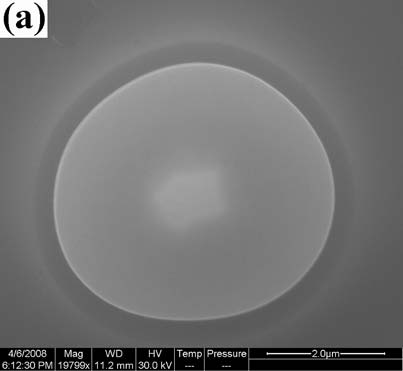
\includegraphics[width=0.40\linewidth]{Figures/Cao1.png}
    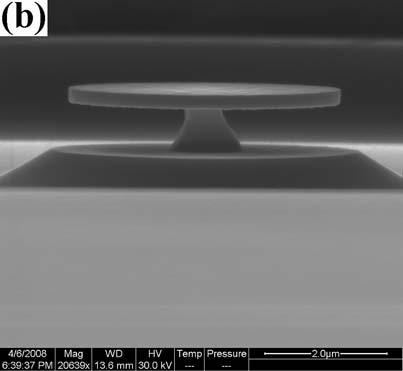
\includegraphics[width=0.40\linewidth]{Figures/Cao2.png}
  \end{center}

  {\footnotesize{Q. H. Song \emph{et al.}, Phys. Rev. A {\bf 80}, 041807 (2009)}}

\end{frame}


\begin{frame}{Billards: Koordinaten}

  Zwei Freiheitsgrade $\entspricht 4d$-Phasenraum. Reduziere auf \emph{Birkhoff-Koordinaten}:

  \begin{center}
    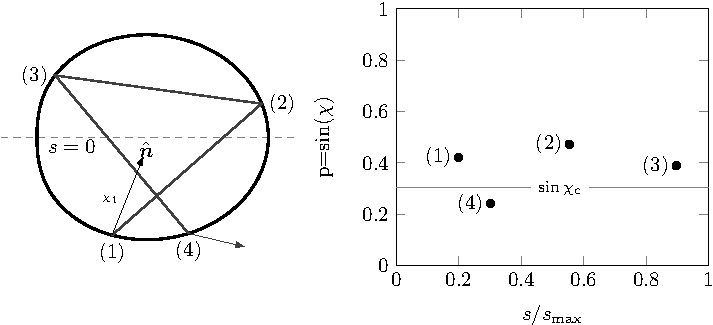
\includegraphics[width=0.95\linewidth]{Figures/Billiard-crop.pdf}
  \end{center}

  Zwischen zwei Reflektionen: geradlinige Bewegung!
\end{frame}


\begin{frame}{Dimensionsreduktion}

  Allgemein: Untersuchung hochdimensionaler Systeme -- Poincar\'e-Schnitte:

  \begin{center}
    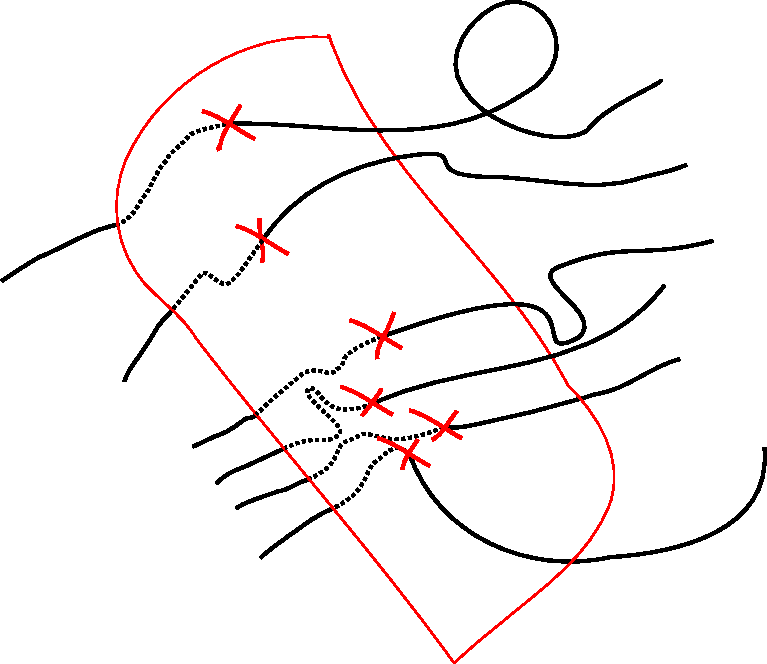
\includegraphics[width=0.55\textwidth]{Figures/PSOS.pdf}
  \end{center}

  Registriere Schnittpunkte von Trajektorie und \emph{Poincar\'e-Schnittebene}
\end{frame}


\begin{frame}{Billards: Übergang reguläre Dynamik $\to$ Chaos}

  Betrachte das Lima\c{c}on von Pascal: $r(\phi) = R + \epsilon\cos(\phi)$\\[0.5ex]
  $\leadsto$ \alert{Simulation}: Übergang reguläre Dynamik $\to$ Chaos\\[1ex]

  \only<2>{
    \begin{center}
      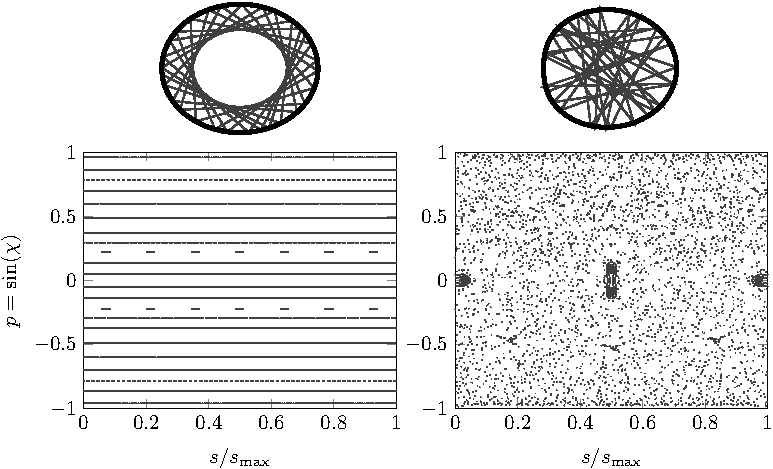
\includegraphics[width=0.85\textwidth]{Figures/Phasenraumbilder-crop.pdf}
  \end{center}}
\end{frame}


\begin{frame}{Konzept: der Lyapunov-Exponent}

  Wie sehr zwei benachbarte Trajektorien mit den Anfangsbedingungen $\vec\xi_0$ und $\vec\xi_0 + \delta\vec\xi_0$ auseinander laufen, kann quantifiziert werden:

  \begin{alertbbox}{Der Lyapunov-Exponent}
    Idee: eine kleine anfängliche  Störung $\delta\vec\xi_0$ wächst gemäß
    \[\abs{\delta\vec\xi(t)} = \eto{\lambda t}\abs{\delta\vec\xi_0}\,.\]
    Für jede Dimension des Systems gibt es einen Lyapunov-Exponenten $\lambda$.
  \end{alertbbox}
  \begin{itemize}
  \item $\lambda > 0$: exponentielles Auseinanderlaufen
  \item $\lambda < 0$: exponentielles Zusammenlaufen
  \item $\lambda = 0$: benachbart bleiben
  \end{itemize}
\end{frame}


\begin{frame}{Lyapunov-Exponent II}

  Eigenschaften:
  \begin{itemize}
  \item konservatives System: $\sum_i \lambda_i = 0$ (\emph{Satz von Liouville})
  \item dissipatives System: $\sum_i \lambda_i < 0$
  \end{itemize}

  \begin{exbox}{Berechnung des maximalen Lyapunov-Exponenten}
    \[\lambda = \lim\limits_{t\to\infty}\lim\limits_{\delta\vec\xi_0 \to \vec 0} \frac{1}{t}\ln\frac{\abs{\delta\vec\xi(t)}}{\abs{\delta\vec\xi_0}}\]
  \end{exbox}

  \begin{exbox}{Konzept: lokaler Lyapunov-Exponent}
    Expansion/Schrumpfung einer kleinen Kugel von Anfangsbedingungen um ein $\vec\xi_0$
    ist gegeben durch die Eigenwerte der Jacobi-Matrix $\partial\vec f/\partial \vec \xi\vert_{\vec\xi_0}$
    (mit $\vec f$ dem Fluß/der Abbildung).
  \end{exbox}
\end{frame}


\begin{frame}{Abhängigkeit von Anfangsbedingungen -- \emph{revisited}}

  Betrachte für das reguläre Lima\c{c}on mit $\epsilon=0.2$ einen kleinen Kreis von Anfangsbedingungen:

  \only<1>{
    \begin{center}
      \includegraphics[width=0.65\textwidth]{Figures/{Lim_eps0.2_iteration0}.png}
  \end{center}}

  \only<2>{
    \begin{center}
      \includegraphics[width=0.65\textwidth]{Figures/{Lim_eps0.2_iteration1}.png}
  \end{center}}

  \only<3>{
    \begin{center}
      \includegraphics[width=0.65\textwidth]{Figures/{Lim_eps0.2_iteration2}.png}
  \end{center}}

  \only<4>{
    \begin{center}
      \includegraphics[width=0.65\textwidth]{Figures/{Lim_eps0.2_iteration7}.png}
  \end{center}}

  \only<5>{
    \begin{center}
      \includegraphics[width=0.65\textwidth]{Figures/{Lim_eps0.2_iteration19}.png}
  \end{center}}

  \only<6>{
    \begin{center}
      \includegraphics[width=0.65\textwidth]{Figures/{Lim_eps0.2_iteration40}.png}
  \end{center}}

  \only<7>{
    \begin{center}
      \includegraphics[width=0.65\textwidth]{Figures/{Lim_eps0.2_iteration99}.png}
  \end{center}}
\end{frame}


\begin{frame}{Abhängigkeit von Anfangsbedingungen -- \emph{revisited}}

  Betrachte nun das chaotische Lima\c{c}on mit $\epsilon=0.45$ ebenfalls einen
  kleinen Kreis von Anfangsbedingungen:

  \only<1>{
    \begin{center}
      \includegraphics[width=0.65\textwidth]{Figures/{Lim_eps0.45_iteration0}.png}
  \end{center}}

  \only<2>{
    \begin{center}
      \includegraphics[width=0.65\textwidth]{Figures/{Lim_eps0.45_iteration1}.png}
  \end{center}}

  \only<3>{
    \begin{center}
      \includegraphics[width=0.65\textwidth]{Figures/{Lim_eps0.45_iteration4}.png}
  \end{center}}

  \only<4>{
    \begin{center}
      \includegraphics[width=0.65\textwidth]{Figures/{Lim_eps0.45_iteration6}.png}
  \end{center}}

  \only<5>{
    \begin{center}
      \includegraphics[width=0.65\textwidth]{Figures/{Lim_eps0.45_iteration9}.png}
  \end{center}}

  \only<6>{
    \begin{center}
      \includegraphics[width=0.65\textwidth]{Figures/{Lim_eps0.45_iteration11}.png}
  \end{center}}

  \only<7>{
    \begin{center}
      \includegraphics[width=0.65\textwidth]{Figures/{Lim_eps0.45_iteration15}.png}
  \end{center}}

  \only<8>{
    \begin{center}
      \includegraphics[width=0.65\textwidth]{Figures/{Lim_eps0.45_iteration19}.png}
    \end{center}

    $\leadsto$ \alert{mischende} Dynamik!
  }
\end{frame}
